%% This is file `elsarticle-template-1-num.tex',
%%
%% Copyright 2009 Elsevier Ltd
%%
%% This file is part of the 'Elsarticle Bundle'.
%% ---------------------------------------------
%%
%% It may be distributed under the conditions of the LaTeX Project Public
%% License, either version 1.2 of this license or (at your option) any
%% later version.  The latest version of this license is in
%%    http://www.latex-project.org/lppl.txt
%% and version 1.2 or later is part of all distributions of LaTeX
%% version 1999/12/01 or later.
%%
%% Template article for Elsevier's document class `elsarticle'
%% with numbered style bibliographic references
%%
%% $Id: elsarticle-template-1-num.tex 149 2009-10-08 05:01:15Z rishi $
%% $URL: http://lenova.river-valley.com/svn/elsbst/trunk/elsarticle-template-1-num.tex $
%%
\documentclass[preprint,12pt]{elsarticle}

\usepackage[colorlinks]{hyperref}
\usepackage[colorinlistoftodos]{todonotes}
\usepackage{verbatim}

%% Use the option review to obtain double line spacing
%% \documentclass[preprint,review,12pt]{elsarticle}

%% Use the options 1p,twocolumn; 3p; 3p,twocolumn; 5p; or 5p,twocolumn
%% for a journal layout:
%% \documentclass[final,1p,times]{elsarticle}
%% \documentclass[final,1p,times,twocolumn]{elsarticle}
%% \documentclass[final,3p,times]{elsarticle}
%% \documentclass[final,3p,times,twocolumn]{elsarticle}
%% \documentclass[final,5p,times]{elsarticle}
%% \documentclass[final,5p,times,twocolumn]{elsarticle}

%% The graphicx package provides the includegraphics command.
\usepackage{graphicx}
%% The amssymb package provides various useful mathematical symbols
\usepackage{amssymb}
%% The amsthm package provides extended theorem environments
%% \usepackage{amsthm}

%% The lineno packages adds line numbers. Start line numbering with
%% \begin{linenumbers}, end it with \end{linenumbers}. Or switch it on
%% for the whole article with \linenumbers after \end{frontmatter}.
\usepackage{lineno}

%% natbib.sty is loaded by default. However, natbib options can be
%% provided with \biboptions{...} command. Following options are
%% valid:

%%   round  -  round parentheses are used (default)
%%   square -  square brackets are used   [option]
%%   curly  -  curly braces are used      {option}
%%   angle  -  angle brackets are used    <option>
%%   semicolon  -  multiple citations separated by semi-colon
%%   colon  - same as semicolon, an earlier confusion
%%   comma  -  separated by comma
%%   numbers-  selects numerical citations
%%   super  -  numerical citations as superscripts
%%   sort   -  sorts multiple citations according to order in ref. list
%%   sort&compress   -  like sort, but also compresses numerical citations
%%   compress - compresses without sorting
%%
%% \biboptions{comma,round}

% \biboptions{}

\journal{DAACH}

\begin{document}

\begin{frontmatter}

%% Title, authors and addresses

\title{3D Scan Data for Selected Clovis-Age Artifacts from the Gault Site (41BL323), Central Texas, USA}

%% use the tnoteref command within \title for footnotes;
%% use the tnotetext command for the associated footnote;
%% use the fnref command within \author or \address for footnotes;
%% use the fntext command for the associated footnote;
%% use the corref command within \author for corresponding author footnotes;
%% use the cortext command for the associated footnote;
%% use the ead command for the email address,
%% and the form \ead[url] for the home page:
%%
%% \title{Title\tnoteref{label1}}
%% \tnotetext[label1]{}
%% \author{Name\corref{cor1}\fnref{label2}}
%% \ead{email address}
%% \ead[url]{home page}
%% \fntext[label2]{}
%% \cortext[cor1]{}
%% \address{Address\fnref{label3}}
%% \fntext[label3]{}


%% use optional labels to link authors explicitly to addresses:
%% \author[label1,label2]{<author name>}
%% \address[label1]{<address>}
%% \address[label2]{<address>}
\author{Robert Z. Selden Jr.\textsuperscript{1}*, Thomas J. Williams\textsuperscript{2, 3}, Nancy Velchoff\textsuperscript{2, 3} and Michael B. Collins\textsuperscript{2, 3}} % Authors
\address{\textsuperscript{1}\textit{Heritage Research Center, Stephen F. Austin State University, USA}} % Author affiliation
\address{\textsuperscript{3}\textit{Prehistory Research Project, Department of Anthropology, Texas State University, USA}}%
\address{\textsuperscript{4}\textit{Gault School of Archaeological Research, San Marcos, Texas, USA}}

\begin{abstract}
%% Text of abstract
On August 19, 2016, selected Clovis artifacts from the Gault site (41BL323) were scanned in advance of a large collaborative research project. These data were collected using a NextEngineHD running ScanStudioHD Pro, and were post-processed in Geomagic Design X 2016.0.1. All data associated with this project have been made publicly available (open access) and are accessible in Zenodo under a Creative Commons Attribution license, where they can be downloaded for use in additional projects and learning activities. These data have the capacity to augment a variety of research designs spanning the digital humanities, applications of geometric morphometrics, and many others. Additionally, these scans will augment a wide range of comparative research topics throughout the Americas and beyond. Reuse potential for these data is significant.
\end{abstract}

\begin{keyword}
Clovis \sep Projectile Points \sep 3D \sep The Gault Site
%% keywords here, in the form: keyword \sep keyword

%% MSC codes here, in the form: \MSC code \sep code
%% or \MSC[2008] code \sep code (2000 is the default)

\end{keyword}

\end{frontmatter}

%%
%% Start line numbering here if you want
%%
\linenumbers

%% main text
\section{Overview} % The \section*{} command stops section numbering
The Gault Site (41BL323), located in Central Texas, USA (Figure ~\ref{fig:Fig1}), is a large, open-air site with an extensive, stratified sequence encompassing a near-complete regional prehistoric sequence. Dense deposits of Clovis-age stone tools,  manufacturing debris, and associated faunal material (e.g., mammoth, horse, and bison) have been systematically excavated from the site\cite{Collins2002}. Overall, the Gault Clovis assemblage is comprised of approximately 600,000 artifacts, around ninety-five percent being lithic material; most recovered from nine major excavation blocks from less then three percent of the entire site. Recently published studies of the Gault Clovis materials include an analysis of incised stones \cite{Lemke2015}, Clovis blade technology \cite{Williams2016}, Clovis Flake analysis \cite{Velchoff2015}, and Optically Stimulated Luminescence ages of the Clovis component in Area 15 \cite{Rodrigues2016}. Current analytical investigations include microscopic use-wear, geomorphological, paleomagnetic, microfossil, and starch grain analyses. Other investigations include the identification of family and/or species from fragmented faunal remains using ZooMS (Zooarchaeology by Mass Spectrometry) \cite{KeenanEarly2016,Buckley2008}. 

\begin{figure}[ht]\centering
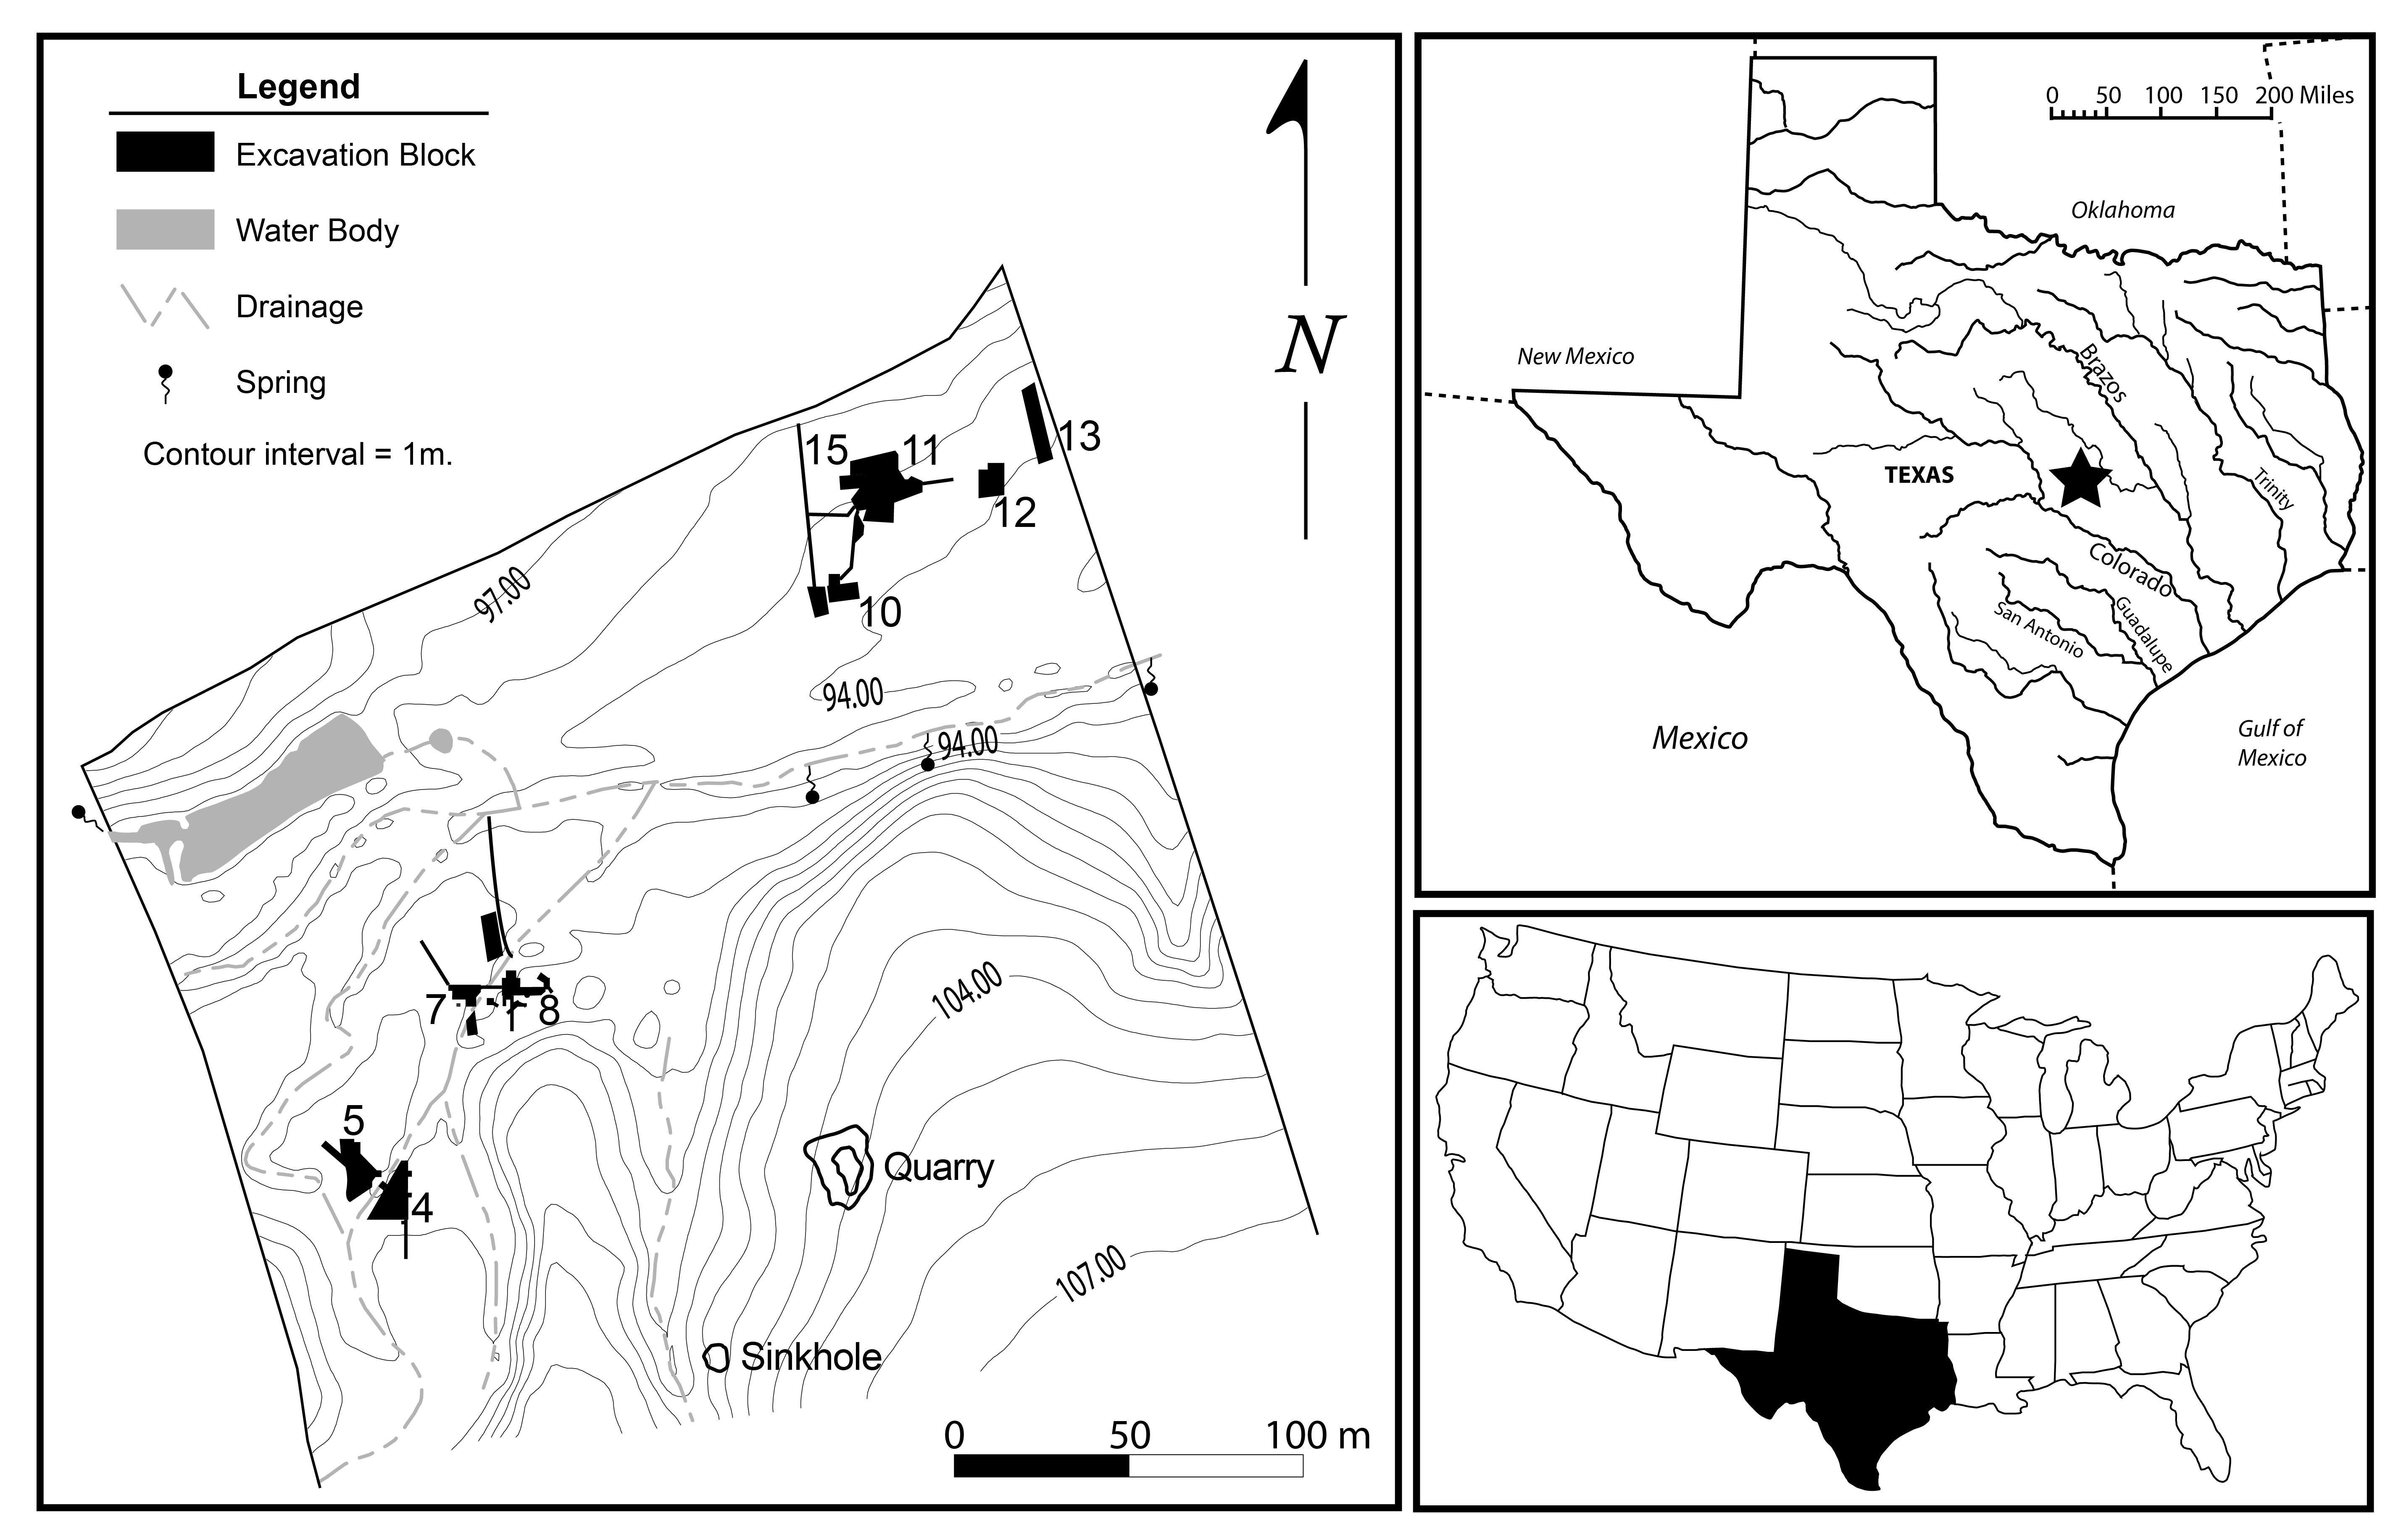
\includegraphics[width=\linewidth]{Fig_1}
\caption{Map of the Gault site indicating those areas where Clovis-age deposits were discovered. The 3D scanned Clovis points were recovered from areas 4, 7, and 8.}
\label{fig:Fig1}
\end{figure}

\begin{figure}[th]\centering

\includegraphics[width=\linewidth]{Fig2}
\caption{3D scan of GAULT 41BL323 LOT1040-113. \em This is a 3D figure that can be rotated, measured and otherwise quantified. To activate the figure, this article must be downloaded to your computer. Activate the figure by clicking on the image, then click/drag to rotate.}
\label{fig:Fig2}
\end{figure}

Lithic analysis remains ongoing and the addition of other analytical approaches, in this case, that employ 3D meshes helps to advance discussions of shape variation that occurs among these artifacts; many of which are regularly used in studies of shape using 2D data  \cite{RN256, RN258, RN4570, RN1812, RN4589}. There are many components of shape that are difficult--if not impossible--to characterize using traditional orthogonal approaches \cite{Shott:1, Shott:2}, and are more accurately captured and analyzed in their native 3D format \cite{RN4546, RN4561}. These attributes can be couched in a variety of theoretical frameworks \cite{Hosfield:1, Costin:1, Costin:2}; however, evolutionary archaeology remains \textit{de rigueur} for geometric morphometric studies of lithic artifacts \cite{Lycett2015}. While the production of 3D data are labor and time-intensive (although see \cite{Ahmed:1}), the benefits can be seen in their contribution to conservation \cite{Kuzminsky:1}, participatory digital archaeology \cite{Morgan:1}, and dynamic illustrations \cite{Magnani:1, Carlson:1}. Furthermore, with the ability to convert these 3D scans (Figure ~\ref{fig:Fig2}) into printed replicas, new avenues in public outreach and education can be explored \cite{Means2013}.

\subsection{Context}
While the detailed context of these artifacts is discussed elsewhere \cite{Collins2002,Collins2007,Bradley2010,Rodrigues2016,Speer2014,Waters2011}, an abbreviated listing is included in Table ~\ref{tab:Tbl1}, and in each of the Zenodo entries. Three Clovis points were recovered from Area 8 (2621-1, 36-42, and 191-174). Two further points, 2643-15 and 1323-1, were recovered from areas seven and four respectively. Finally, Clovis points 2624-1 and 1040-113 were recovered from the surface.

\begin{table}[tbh]\centering
\caption{Context of Scanned Artifacts}
\centering
\begin{tabular}{lll}
\hline
Artifact No. & Description & Provenience \\
\hline
2621-1 & Clovis Pt & Area 8\\
36-42 & Clovis Pt & Area 8\\
2643-15 & Clovis Pt & Area 7\\
191-174 & Clovis Pt & Area 8\\
2624-1 & Clovis Pt & Surface\\
1323-1 & Clovis Pt & Area 4\\
1040-113 & Clovis Pt & Surface (Area 8)\\
\hline
\end{tabular}
\label{tab:Tbl1}
\end{table}

\subsection{Temporal Coverage} 

To date, a total of six luminescence ages associated with the Clovis deposits have been reported; four from Area 15 \cite{Rodrigues2016}, and two from Area 8 \cite{Waters2011}. These ages fit within the known age range for the Clovis period, approximately 13,500 to 12,800 cal BP \cite{Holliday2000,Meltzer2009} (Figure ~\ref{fig:Fig3}). 

\begin{figure}[ht]\centering
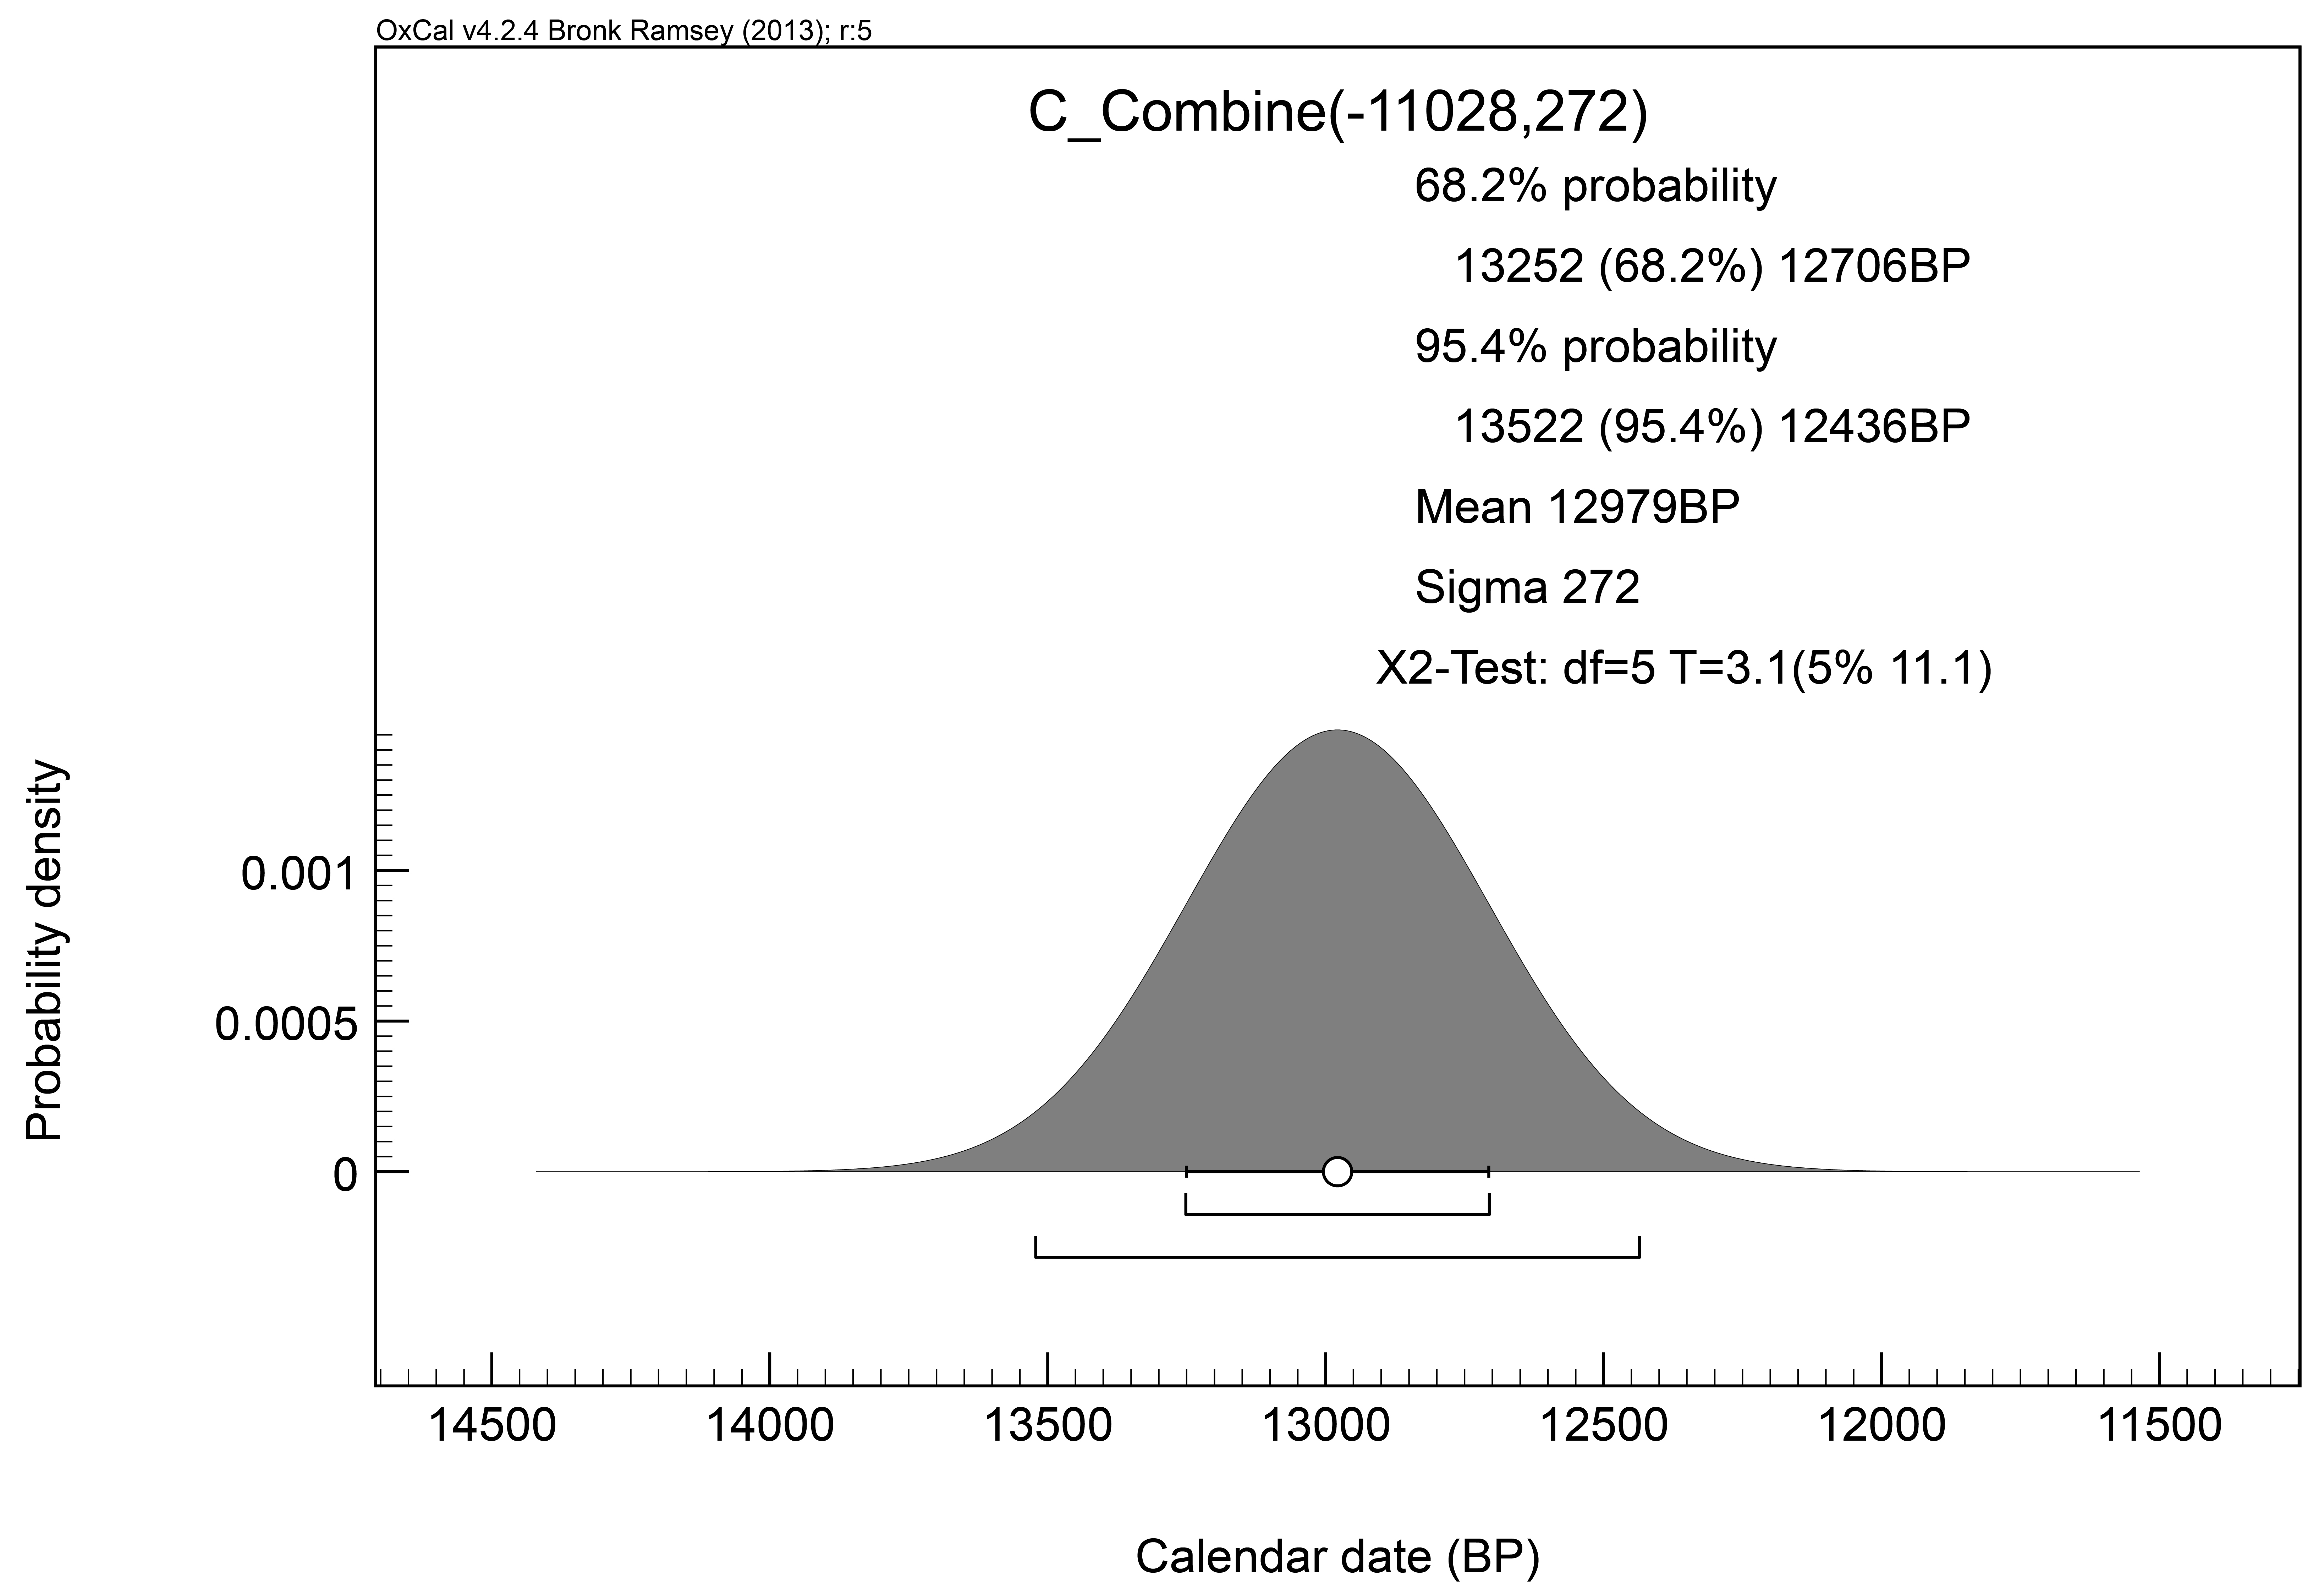
\includegraphics[width=\linewidth]{Fig3}
\caption{Luminescence age range associated with the Clovis-age deposits from the Gault Site. All dates (\textit{n} = 6) were combined using the C\_Combine function in OxCal v.4.2.4 \citep{RN308}.}
\label{fig:Fig3}
\end{figure}

%------------------------------------------------

\section{Methods}

Selected artifacts were scanned using a NextEngineHD running ScanStudioHD Pro. Scan data were collected at the highest HD setting using eight divisions, then trimmed, aligned, fused and polished in ScanStudioHD Pro before being exported as ASCII.stl and ASCII.ply files prior to post-processing \cite{Galeazzi:1,Weyrich:1}. Those data were then imported into Geomagic Design X, where the final meshes were aligned and processed.

\subsection{Steps}

To align each scan, a reference vector was inserted, followed by a reference point at the confluence of the vector and the mesh (using a projection) at the central base. A plane was inserted using the pick point and normal axis function, utilizing the vector as the normal axis, and the projected point as the pick point. Both elements (reference vector and reference point) of reference geometry were then utilized in an interactive alignment, with the the reference vector as the moving vector, and the reference point as the moving point (Figure ~\ref{fig:Fig2}). Alignment has proven to be an important factor in downstream analyses, particularly when making the transition from Design X and Control to SolidWorks or other CAD-based platform \cite{Selden:5} like those used to generate the 3D puzzles (Figure ~\ref{fig:Fig4}). 

\begin{figure}[ht]\centering
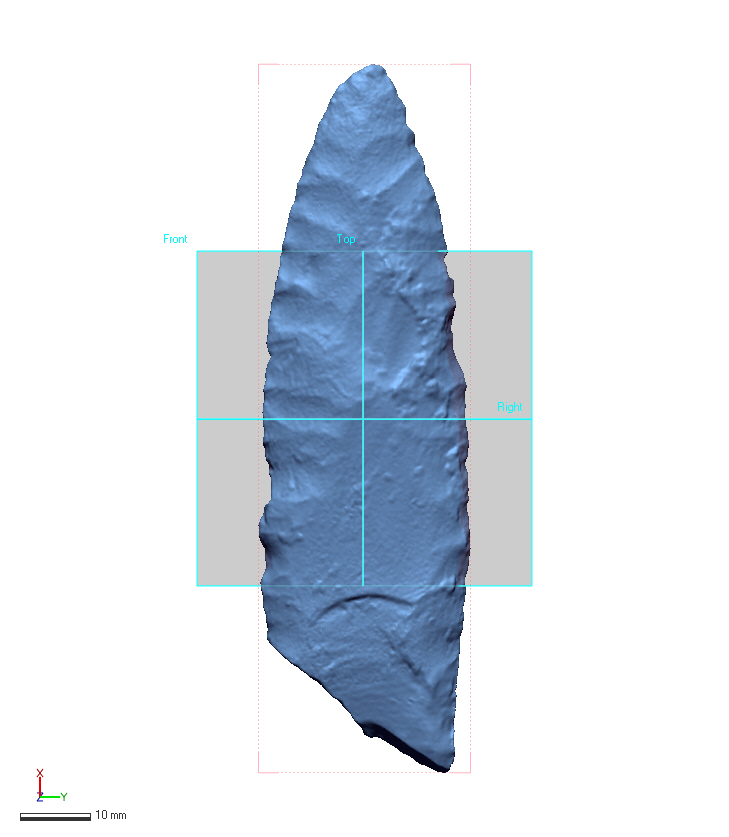
\includegraphics[width=0.85\linewidth]{Fig4}
\caption{Aligned 3D mesh for GAULT 41BL323 LOT1040-113 showing reference planes.}
\label{fig:Fig4}
\end{figure}

Post-processing of each 3D mesh began with the healing wizard function in Design X, correcting problematic issues with non-manifold poly-vertices, folded poly-faces, dangling poly-faces, small clusters, small poly-faces, non-manifold poly-faces, crossing poly-faces, and small tunnels. The rewrap function was then used to render the final mesh. Upon completion of post-processing, each mesh was decimated by 50 percent prior to saving then export as an ASCII.ply. Decimation of the mesh decreases file size while increasing ease of use on standard computers.

\subsection{3D Puzzles}

In addition to the 3D models, one 3D cardboard puzzle was created (for GAULT 41BL323 LOT1040-113 \cite{Selden:Z27}) to augment the on-site efforts of the interpretive staff by providing a physical model through which visitors can interact with the digital proxy. These cardboard puzzles were generated using Autodesk 123D Make \cite{Autodesk:1}, and the plans for the cardboard puzzles (Figure ~\ref{fig:Fig5}) accompanied the uploads to Zenodo. Those plans can be downloaded, glued to cardboard, then cut out to create a tangible model of a Clovis point. These files were uploaded to Zenodo in .pdf format, and are also compatible with most laser cutters.

\begin{figure}[ht]\centering
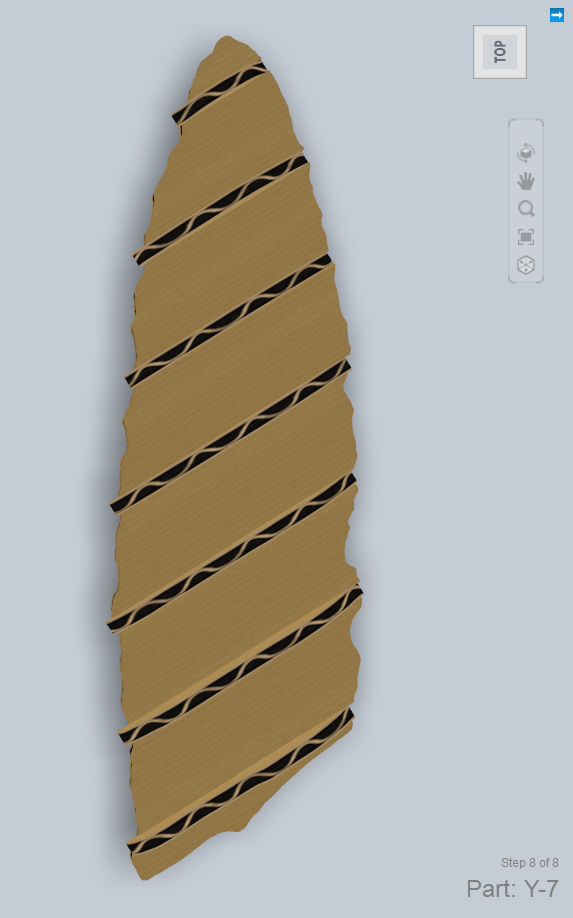
\includegraphics[width=0.95\linewidth]{Fig5}
\caption{Modeled 3D puzzle of GAULT 41BL323 Lot1040-113 \cite{Selden:Z27} created with Autodesk 123D Make at a uniform scale.}
\label{fig:Fig5}
\end{figure}

\section{Data Description}

\subsection{Collection Name}

3D Scans from the Gault Site

\subsection{Data Type}

Decimated meshes

\subsection{Format Names and Versions}

ASCII.ply (mesh)

\subsection{Creation Date}

August 19, 2016

\subsection{Dataset Creator}

Robert Z. Selden Jr.

\subsection{Language}

English

\subsection{License}

Creative Commons Attribution

\subsection{Repository Location}
3D Scans from the Gault Site

\begin{itemize}

\item GAULT 41BL323 LOT2621-1 \citep{Selden:Z21}

\item GAULT 41BL323 LOT36-42 \citep{Selden:Z25}

\item GAULT 41BL323 LOT2643-15 \citep{Selden:Z24}

\item GAULT 41BL323 LOTAM191-174 \citep{Selden:Z23}

\item GAULT 41BL323 LOT2624-1 \citep{Selden:Z22}

\item GAULT 41BL323 LOTNH1323-1 \citep{Selden:Z20}

\item GAULT 41BL323 LOT1040-113 \citep{Selden:Z26}

\end{itemize}

\subsection{Data Publication Date}

October 31, 2016

\section{Reuse Potential}

Those data from this project have long-term and wide-ranging reuse potential, of which many applications may (likely) not yet have been contemplated. While the primary purpose of this endeavor was to document these resources for use in additional analytical and outreach efforts, one of the projectile points has since been modeled as a 3D puzzle that can be cut out using materials that are easily acquired by most (i.e., a cardboard box). 

These data have significant reuse potential in the sciences and digital humanities where they can augment both qualitative and quantitative studies. They also hold promise for clarifying questions of the shape, form, size and asymmetry of these artifacts, which can be addressed in analyses of asymmetry and geometric morphometrics. 

%------------------------------------------------
\section*{Acknowledgments}

We extend our gratitude to the Gault School of Archaeological Research and to Texas State University for providing the requisite permissions and access needed to scan this selection of artifacts. We also thank Dr. Loren G. Davis and Dr. Bruce Bradley for their comments on an earlier draft. Research at the Gault Site was funded in part by NSF Grant 0920549 to Texas State University, San Marcos, by The Gault School of Archaeological Research, and by private donors.

The 3D model used in Figure ~\ref{fig:Fig2} was generated as a .ply in Geomagic Design X and converted to a .u3d in DAZ Studio.


%% The Appendices part is started with the command \appendix;
%% appendix sections are then done as normal sections
%% \appendix

%% \section{}
%% \label{}

%% References
%%
%% Following citation commands can be used in the body text:
%% Usage of \cite is as follows:
%%   \cite{key}          ==>>  [#]
%%   \cite[chap. 2]{key} ==>>  [#, chap. 2]
%%   \citet{key}         ==>>  Author [#]

%% References with bibTeX database:

\bibliographystyle{model1-num-names}
\bibliography{sample.bib}

%% Authors are advised to submit their bibtex database files. They are
%% requested to list a bibtex style file in the manuscript if they do
%% not want to use model1-num-names.bst.

%% References without bibTeX database:

% \begin{thebibliography}{00}

%% \bibitem must have the following form:
%%   \bibitem{key}...
%%

% \bibitem{}

% \end{thebibliography}


\end{document}

%%
%% End of file `elsarticle-template-1-num.tex'.